













\begin{figure}[]
\setlength{\abovecaptionskip}{-4pt}
\begin{center}
\includegraphics{Introversion_Extraversion.png}
  \caption{Introversion Extraversion.png}
  \end{center}


{\normalsize{\bf the interpretation:}} \\\vspace{0.5cm}
the representation show that the graph is not symmetric allowing 
the mean wich equal 0.04  for the females and -0.06  for the males 

The result in this case that females are more Introversion/Extraversion than males
\end{figure}


\begin{figure}[]
\setlength{\abovecaptionskip}{-4pt}
\begin{center}
\includegraphics{Neuro.png}
  \caption{Neuro.png}
  \end{center}

{\normalsize{\bf the interpretation:}} \\\vspace{0.5cm}
the representation show that the graph is not symmetric allowing 
the mean witch equal 0.14 for the females and -0.22 for the males 

The result in this case that females are more Neuro  than males
\end{figure}

\begin{figure}[]
\setlength{\abovecaptionskip}{-4pt}
\begin{center}
\includegraphics{Agree.png}
  \caption{Agree.png}
  \end{center}

{\normalsize{\bf the interpretation:}} \\\vspace{0.5cm}
the representation show that the graph is not symmetric allowing 
the mean witch equal 0,18 for the females and -0.27 for the males

The result in this case that females are more Agree  than males
\end{figure}

\begin{figure}[]
\setlength{\abovecaptionskip}{-4pt}
\begin{center}
  \includegraphics{openess.png} 
  \caption{openess.png}
\end{center}

{\normalsize{\bf the interpretation:}} \\\vspace{0.5cm}
the representation show that the graph is not symmetric allowing 
the mean witch equal 0.036 for the females and -0.054 for the males

The result in this case that females are Openess than males
\end{figure}

\begin{figure}[]
\setlength{\abovecaptionskip}{-4pt}
\begin{center}
\includegraphics{Conscient.png}
  \caption{Conscient.png}
  \end{center}


{\normalsize{\bf the interpretation:}} \\\vspace{0.5cm}
the representation show that the graph is not symmetric allowing 
the mean wich equal -0.092 for the females and 0.14 for the males

The result in this case that males are  more Consient  than females

\end{figure}
\begin{figure}[]
\setlength{\abovecaptionskip}{-4pt}
\begin{center}
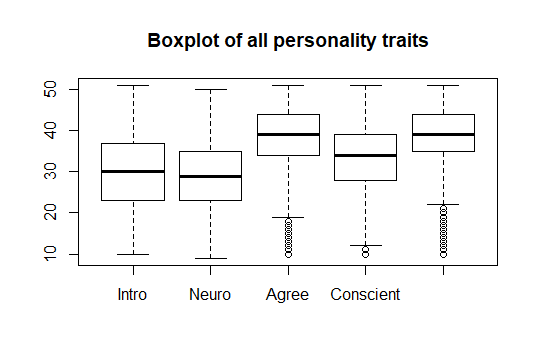
\includegraphics{Boxplot_of_all_personality.png}
  \caption{Boxplot of allpersonality.png}
  \end{center}


{\normalsize{\bf the interpretation:}} \\\vspace{0.5cm}
we observe that the boxplots of introverted/extroverted persons and neuro (isolated) are larger than agreer and opened persons 

\end{figure}






